%% TWO SLIT - UNOBSEVRED, EXPECTED, PARTICLE-LIKE BEHAVIOUR WITH ELECTRON GUN

% https://tikz.net/optics_twoslit/
% https://www.overleaf.com/learn/latex/Counters
% https://tex.stackexchange.com/questions/29989/how-does-the-counter-in-tikz-foreach-work
% https://tex.stackexchange.com/questions/45848/rotate-node-text-and-use-relative-positioning-in-tikz
% https://tex.stackexchange.com/questions/625022/using-tikz-to-plot-angle-notations-and-various-arrows
% https://tex.stackexchange.com/questions/449675/how-to-draw-a-coil-such-that-you-can-see-if-its-right-or-left-handed
\documentclass{standalone}


% https://tikz.net/optics_twoslit/
% https://www.overleaf.com/learn/latex/Counters
% https://tex.stackexchange.com/questions/29989/how-does-the-counter-in-tikz-foreach-work
% https://tex.stackexchange.com/questions/45848/rotate-node-text-and-use-relative-positioning-in-tikz
% https://tex.stackexchange.com/questions/625022/using-tikz-to-plot-angle-notations-and-various-arrows
% https://tex.stackexchange.com/questions/449675/how-to-draw-a-coil-such-that-you-can-see-if-its-right-or-left-handed



\IfStandalone{\def\datapath{../../../}}{\def\datapath{}}


\IfStandalone{\def\datapath{../../../}}{\def\datapath{}}

\usepackage{xcolor}
\definecolor{SciencePurple}{HTML}{663399}
\definecolor{ScienceBlue}{HTML}{214CCE}
\definecolor{ScienceGreen}{HTML}{007510}
\definecolor{ScienceYellow}{HTML}{ffbf00}
\definecolor{ScienceOrange}{HTML}{ff8c00}
\definecolor{ScienceRed}{HTML}{dc143c}
\usepackage{fontspec}
	\setmainfont{Roboto Slab}
	\setsansfont{Lato}
	\renewcommand{\familydefault}{\sfdefault}
	\setlength{\intextsep}{4pt} % Set defualt spacing around floats
	\definecolor{CommentGreen}{HTML}{228B22}
%	\captionsetup{aboveskip=5pt, belowskip=5pt} % Reduce space around captions

%% Math Env Text Settings
\usepackage{mathtools}
\usepackage{unicode-math}
	\setmathfont{XITS Math}
\usepackage{amsmath}
\usepackage{bm}
%	\everymath=\expandafter{\the\everymath\displaystyle}


%% https://tex.stackexchange.com/questions/8434/how-to-scale-math-font-only#8448
\DeclareMathSizes{11pt}{12pt}{7pt}{7pt}
\DeclareMathSizes{14pt}{15pt}{9pt}{9pt}

%% https://tex.stackexchange.com/questions/122574/globally-changing-math-line-spacing
\setlength{\jot}{7pt}

%% https://www.overleaf.com/learn/latex/Spacing_in_math_mode
%% https://tex.stackexchange.com/questions/41913/how-to-get-less-spacing-in-math-mode
%% https://mirror.kumi.systems/ctan/obsolete/info/math/voss/mathmode/Mathmode.pdf
\thinmuskip=5mu % (by default it is equal to 3 mu)
\medmuskip=5mu  % (by default it is equal to 4 mu)
\thickmuskip=7mu  % (by default it is equal to 5 mu)


\usepackage{tikz}
\usepackage{siunitx}
\usepackage{pgfplots}

\usepackage{physics}
\usepackage{etoolbox} %ifthen
\usepackage[outline]{contour} % glow around text


%%%%%%%%%% PGFPLOTS & PGFPLOTS SETTINGS %%%%%%%%%%
\pgfplotsset{compat=newest,
	width=6cm,
	height=3cm,
	scale only axis=true,
	max space between ticks=25pt,
	try min ticks=5,
	every axis/.style={
		axis y line=left,
		axis x line=bottom,
		axis line style={thick,->,>=latex, shorten >=-.4cm}
	},
	every axis plot/.append style={thick},
	tick style={black, thick}
}
\tikzset{
	semithick/.style={line width=0.8pt},
}

\usepgfplotslibrary{groupplots}
\usepgfplotslibrary{dateplot}


\usetikzlibrary{calc}
\usetikzlibrary{arrows,arrows.meta,math}
\usetikzlibrary{decorations.markings}
\usetikzlibrary{angles,quotes} % for pic (angle labels)
\usetikzlibrary{fadings}
\tikzset{>=latex} % for LaTeX arrow head
\contourlength{1.4pt}

\colorlet{myshadow}{blue!30!black!90}
\tikzstyle{wave}=[ScienceBlue,thick]
\tikzstyle{mydashed}=[black!70,dashed,thin]
\tikzstyle{mymeas}=[{Latex[length=3,width=2]}-{Latex[length=3,width=2]},thin]
\tikzstyle{mysmallarr}=[-{Latex[length=3,width=2]}]

\usetikzlibrary{decorations.pathmorphing}

\newcommand\rightAngle[4]{
	\pgfmathanglebetweenpoints{\pgfpointanchor{#2}{center}}{\pgfpointanchor{#3}{center}}
	\coordinate (tmpRA) at ($(#2)+(\pgfmathresult+45:#4)$);
	\draw[white,line width=0.6] ($(#2)!(tmpRA)!(#1)$) -- (tmpRA) -- ($(#2)!(tmpRA)!(#3)$);
	\draw[ScienceRed] ($(#2)!(tmpRA)!(#1)$) -- (tmpRA) -- ($(#2)!(tmpRA)!(#3)$);
}
\newcommand\lineend[2]{
	\def\w{0.1} \def\c{30}
	\draw[ScienceGreen] (#1)++(#2:\w) to[out=#2-180-\c,in=#2+\c] (#1)
	to[out=#2+\c-180,in=#2-\c]++ (#2-180:\w);
}
\def\tick#1#2{\draw[thick] (#1) ++ (#2:0.1) --++ (#2-180:0.2)}

% INTERFERENCE FADING
\begin{tikzfadingfrompicture}[name=interference]
	\def\lambd{0.5} % wavelength
	\foreach \r in {1,...,15}
	\foreach \j in {1,...,25}
	\path [line width=\lambd*\j,draw=transparent!0,opacity=0.04]
	(0,0) circle (\lambd*\r); %(0:\r) arc (0:180:\r);
\end{tikzfadingfrompicture}

% INTERFERENCE FADING
\begin{tikzfadingfrompicture}[name=interference]
	\def\lambd{0.5} % wavelength
	\foreach \r in {1,...,15}
	\foreach \j in {1,...,25}
	\path [line width=\lambd*\j,draw=transparent!0,opacity=0.04]
	(0,0) circle (\lambd*\r); %(0:\r) arc (0:180:\r);
\end{tikzfadingfrompicture}


\newcommand\DETECTOR[4]{
	\def\Width{#1}
	\def\Height{#2}
	\def\x{#3}
	\def\y{#4}
	
	\path[draw,shape=coordinate]
	(\x-0.5*\Width,\y-0.5*\Height) coordinate(BotL) 
	(\x+0.5*\Width,\y-0.5*\Height) coordinate(BotR)
	(\x+0.5*\Width,\y+0.5*\Height) coordinate(TopR) 
	(\x-0.5*\Width,\y+0.5*\Height) coordinate(TopL)
	(\x-0.5*\Width,\y+0.15*\Height) coordinate(EntryTop)
	(\x+0.1*\Width,\y+0.15*\Height) coordinate(InnerTop)
	(\x+0.1*\Width,\y-0.15*\Height) coordinate(InnerBot)
	(\x-0.5*\Width,\y-0.15*\Height) coordinate(EntryBot);
	\filldraw[color=black,fill=darkgray!25] (BotL) -- (BotR) -- (TopR) -- (TopL) -- (EntryTop) -- (InnerTop) -- (InnerBot) -- (EntryBot) -- (BotL);
}


\newcommand\DETECTORATSLITTOP[4]{
	\def\Width{#1}
	\def\Height{#2}
	\def\x{#3}
	\def\y{#4}
	
	\path[draw,shape=coordinate]
	(\x-0.5*\Width,\y-0.5*\Height) coordinate(BotL)
	(\x-0.5*\Width,\y+0.5*\Height) coordinate(TopL)
	(\x+0.5*\Width,\y+0.5*\Height) coordinate(TopR) 
	(\x+0.5*\Width,\y-0.5*\Height) coordinate(BotR)
	
	(\x+0.2*\Width,\y-0.5*\Height) coordinate(EntryR)
	(\x+0.2*\Width,\y+0.15*\Height) coordinate(InnerR)
	(\x-0.2*\Width,\y+0.15*\Height) coordinate(InnerL)
	(\x-0.2*\Width,\y-0.5*\Height) coordinate(EntryL);
	\filldraw[color=black,fill=darkgray!25] (BotL) -- (TopL) -- (TopR) -- (BotR) -- (EntryR) -- (InnerR) -- (InnerL) -- (EntryL) -- (BotL);
}


\newcommand\DETECTORATSLITBOTTOM[4]{
	\def\Width{#1}
	\def\Height{#2}
	\def\x{#3}
	\def\y{#4}
	
	\path[draw,shape=coordinate]
	(\x-0.5*\Width,\y+0.5*\Height) coordinate(TopL)
	(\x-0.5*\Width,\y-0.5*\Height) coordinate(BotL)
	(\x+0.5*\Width,\y-0.5*\Height) coordinate(BotR)
	(\x+0.5*\Width,\y+0.5*\Height) coordinate(TopR) 	
	
	(\x+0.2*\Width,\y+0.5*\Height) coordinate(EntryR)
	(\x+0.2*\Width,\y-0.15*\Height) coordinate(InnerR)
	(\x-0.2*\Width,\y-0.15*\Height) coordinate(InnerL)
	(\x-0.2*\Width,\y+0.5*\Height) coordinate(EntryL);
	\filldraw[color=black,fill=darkgray!25] (TopL) -- (BotL) -- (BotR) -- (TopR) -- (EntryR) -- (InnerR) -- (InnerL) -- (EntryL) -- (TopL);
}


% Electron Gun
\newcommand\ElectronGun[4]{
	\def\Width{#1}
	\def\Height{#2}
	\def\x{#3}
	\def\y{#4}
	
	\path[draw,shape=coordinate]
	(\x+0.5*\Width,\y-0.15*\Height) coordinate(ExitBot)
	(\x+0.5*\Width,\y-0.5*\Height) coordinate(BotR)
	(\x-0.5*\Width,\y-0.5*\Height) coordinate(BotL)
	(\x-0.5*\Width,\y+0.5*\Height) coordinate(TopL)
	(\x+0.5*\Width,\y+0.5*\Height) coordinate(TopR) 
	(\x+0.5*\Width,\y+0.15*\Height) coordinate(ExitTop);
	\filldraw[color=black,fill=darkgray!25] (ExitBot) -- (BotR) -- (BotL) -- (TopL) -- (TopR) -- (ExitTop);
	
	\draw[decoration={coil,aspect=0.4,segment length=\Height*3.333,amplitude=\Width*2},decorate,color=ScienceRed,fill=darkgray!25] (\x-0.3*\Height,\y+0.4*\Height) -- (\x-0.3*\Height,\y-0.4*\Height);
	
	\draw[color=ScienceRed] (\x-0.3*\Height,\y+0.4*\Height) -- (\x-\Width*0.6,\y+0.4*\Height);
	\draw[color=ScienceRed] (\x-0.3*\Height,\y-0.4*\Height) -- (\x-\Width*0.6,\y-0.4*\Height);
}






\begin{document}
	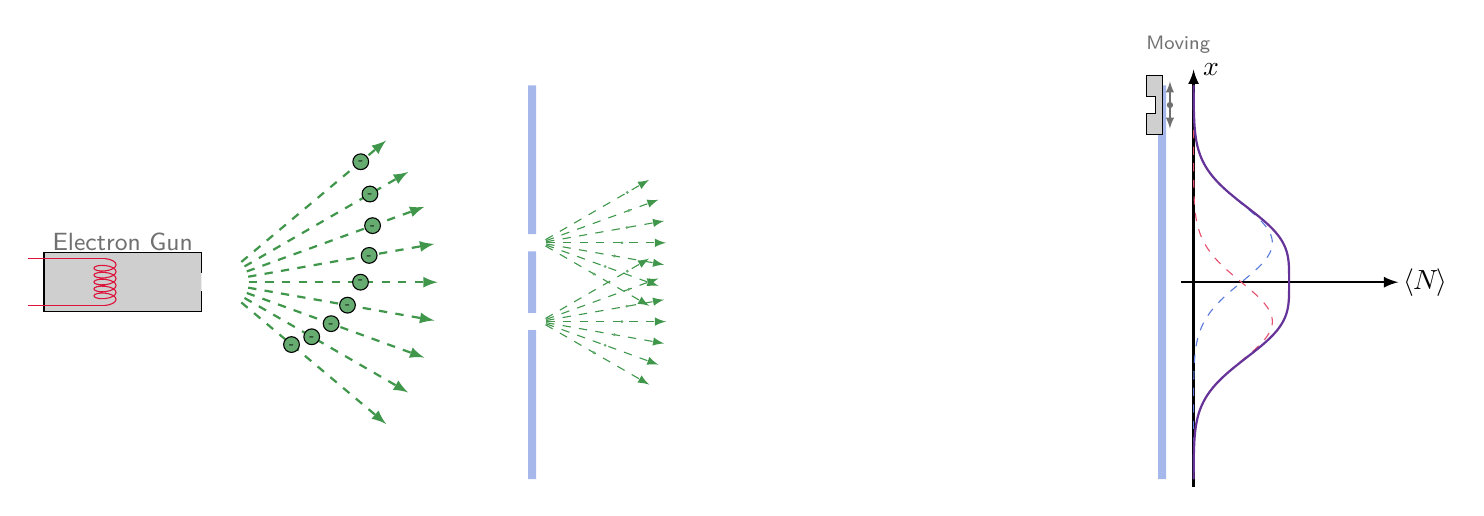
\begin{tikzpicture}[
		nodal/.style={ScienceGreen!50,dashed,thin},
		declare function={
			xMaximaPosition(\Integer) = \ScreenDistL*tan(asin((\Integer*\ScreenDistLambdaDB)/\dSlitSeparationDistance)); % Function to calculate position of screen MAXIMA - "x" in experiment, \y in our tikz diagram - value
			xMinimaPosition(\Integer) = \ScreenDistL*tan(asin(((\Integer+0.5)*\ScreenDistLambdaDB)/\dSlitSeparationDistance)); % Function to calculate position of screen MINIMA - "x" in experiment, \y in our tikz diagram - value
			xRecalculate(\x) = \ScreenDistL-(((\x-\WallTotalSizeinX/2)*\ScreenDistL)/\x); % function to recaluclate - "x" in experiment, \y in our tikz diagram - for maxima/minima in the case we hit the screen out side the limits of the tikz diagram
		}]
		
		\def\ScreenDistL{8}       						% L -- Distance between walls
		\def\WallTotalSizeinX{5}       					% X -- Total wall height
		\def\WallThickness{0.1}      					% t -- wall thickness
		
		\def\dSlitSeparationDistance{1}      			% d -- Centre to centre slit distance
		\def\ScreenDistLambdaDB{0.1}  							% De Broglie Wavelength of electrons
		\def\kVectorNumber{2*3.14159265/\ScreenDistLambdaDB} 		% k -- vectornumber / wavenumber
		
		\def\SlitAperture{0.22}      					% b -- Slit aperture width / size
		
		\pgfmathparse{int(\ScreenDistL/\ScreenDistLambdaDB*2)} % Had to make calculation like this cause tik / pgf was being weird
		\def\NumberOfWavesN{\pgfmathresult}        		% Number of slit emanating and electron gun waves to produce
		
		\def\nMaxAndnMinLinesPerSide{2}					% For doing the right number of MAXIMA/MINIMA lines
		
		\def\ang{60}									% Angle or creating all limited spherical waves
		
		\def\xPositionDetector{0.9}       				% fractional height of projection point, makes point P stand off detector a bit and look neater
		\def\nSamples{1000}								% Number of samples to compute for the intenstiy graph
		
		
		%% Coordinates for the wall
		\coordinate (LeftWallUpper) at (-\WallThickness/2,\WallTotalSizeinX/2);
		\coordinate (LeftWallLower) at (\WallThickness/2,-\WallTotalSizeinX/2);
		
		\coordinate (FirstSlitCentre) at (0,\dSlitSeparationDistance/2);
		\coordinate (FirstSlitUpper) at (\WallThickness/2,\dSlitSeparationDistance/2+\SlitAperture/2);
		\coordinate (FirstSlitLower) at (-\WallThickness/2,\dSlitSeparationDistance/2-\SlitAperture/2);
		
		\coordinate (SecondSlitCentre) at (0,-\dSlitSeparationDistance/2);
		\coordinate (SecondSlitUpper) at (\WallThickness/2,-\dSlitSeparationDistance/2+\SlitAperture/2);
		\coordinate (SecondSlitLower) at (-\WallThickness/2,-\dSlitSeparationDistance/2-\SlitAperture/2);
		
		\coordinate (RightWallUpper) at (\ScreenDistL-\WallThickness/2,\WallTotalSizeinX/2);
		\coordinate (RightWallLower) at (\ScreenDistL+\WallThickness/2,-\WallTotalSizeinX/2);
		
		
		%% WALL
		\fill[ScienceBlue!40]
		(LeftWallUpper) rectangle (FirstSlitUpper)
		(FirstSlitLower) rectangle (SecondSlitUpper)
		(SecondSlitLower) rectangle (LeftWallLower)
		(RightWallUpper) rectangle (RightWallLower);
		
		
		
		%% ELECTRON GUN SYMBOL
		\ElectronGun{2}{0.75}{-\ScreenDistL*0.65}{0}
		\draw[color=darkgray!85] (-\ScreenDistL*0.65,0) node[color=darkgray!75, above = 8] {\small Electron Gun};
		
		%% ELECTRON GUN BEAMS
		%https://wiki.physik.uzh.ch/cms/latex:tikz
		\def\R{\ScreenDistL*0.35} % radius/length of lines
		\def\r{\ScreenDistL*0.05}
		
		\foreach \t/\e/\b in {0/0.65/0.35,10/0.7/0.65,20/0.75/0.72,30/0.8/0.78,40/0.85/0.84)}{
			\draw[->,dashed,ScienceGreen!75,thick]
			({-\ScreenDistL*0.5+\r*cos(\t)},{0+\r*sin(\t)}) -- ({-\ScreenDistL*0.5+\R*cos(\t)},{0+\R*sin(\t)});
			\draw[fill=ScienceGreen!60] ({-\ScreenDistL*0.5+\R*cos(\t)*\e},{0+\R*sin(\t)*\e}) circle [radius = 0.1];
			\node[anchor=center] at ({-\ScreenDistL*0.5+\R*cos(\t)*\e},{0+\R*sin(\t)*\b}) {\tiny -};
		}
		
		\foreach \t/\e/\b in {10/0.6/0.65,20/0.55/0.58,30/0.495/0.515,40/0.44/0.455}{
			\draw[->,dashed,ScienceGreen!75,thick]
			({-\ScreenDistL*0.5+\r*cos(\t)},{0-\r*sin(\t)}) -- ({-\ScreenDistL*0.5+\R*cos(\t)},{0-\R*sin(\t)});
			\draw[fill=ScienceGreen!60] ({-\ScreenDistL*0.5+\R*cos(\t)*\e},{0-\R*sin(\t)*\e}) circle [radius = 0.1];
			\node[anchor=center] at ({-\ScreenDistL*0.5+\R*cos(\t)*\e},{0-\R*sin(\t)*\b}) {\tiny -};
		}
		
		
		
		%% ELECTRON BEAMS FROM SLIT ONE
		%https://wiki.physik.uzh.ch/cms/latex:tikz
		\def\R{\ScreenDistL*0.2} % radius/length of lines
		\def\r{\ScreenDistL*0.01}
		
		\foreach \t/\e/\b in {0/0.65/0.35,10/0.7/0.65,20/0.75/0.72,30/0.8/0.78}{
			\draw[->,dashed,ScienceGreen!75]
			({0.1+\r*cos(\t)},{\dSlitSeparationDistance/2+\r*sin(\t)}) -- ({0.1+\R*cos(\t)},{\dSlitSeparationDistance/2+\R*sin(\t)});
			\draw[fill=ScienceGreen!60,ScienceGreen!60] ({0.1+\R*cos(\t)*\e},{\dSlitSeparationDistance/2+\R*sin(\t)*\e}) circle [radius = 0.01];
		}
		
		\foreach \t/\e/\b in {10/0.6/0.65,20/0.55/0.58,30/0.495/0.515}{
			\draw[->,dashed,ScienceGreen!75]
			({0.1+\r*cos(\t)},{\dSlitSeparationDistance/2-\r*sin(\t)}) -- ({0.1+\R*cos(\t)},{\dSlitSeparationDistance/2-\R*sin(\t)});
			\draw[fill=ScienceGreen!60,ScienceGreen!60] ({0.1+\R*cos(\t)*\e},{\dSlitSeparationDistance/2-\R*sin(\t)*\e}) circle [radius = 0.01];
		}
		
		
		\foreach \t/\e/\b in {0/0.65/0.35,10/0.7/0.65,20/0.75/0.72,30/0.8/0.78}{
			\draw[->,dashed,ScienceGreen!75]
			({0.1+\r*cos(\t)},{-\dSlitSeparationDistance/2+\r*sin(\t)}) -- ({0.1+\R*cos(\t)},{-\dSlitSeparationDistance/2+\R*sin(\t)});
			\draw[fill=ScienceGreen!60,ScienceGreen!60] ({0.1+\R*cos(\t)*\e},{-\dSlitSeparationDistance/2+\R*sin(\t)*\e}) circle [radius = 0.01];
		}
		
		\foreach \t/\e/\b in {10/0.6/0.65,20/0.55/0.58,30/0.495/0.515}{
			\draw[->,dashed,ScienceGreen!75]
			({0.1+\r*cos(\t)},{-\dSlitSeparationDistance/2-\r*sin(\t)}) -- ({0.1+\R*cos(\t)},{-\dSlitSeparationDistance/2-\R*sin(\t)});
			\draw[fill=ScienceGreen!60,ScienceGreen!60] ({0.1+\R*cos(\t)*\e},{-\dSlitSeparationDistance/2-\R*sin(\t)*\e}) circle [radius = 0.01];
		}
		
		
		
		
		% EXPECTED INTENSITY FUNCTION PLOT
		\begin{scope}[shift={(1.05*\ScreenDistL,0)}]
			
			\pgfkeys{/pgf/trig format=rad} %% Took me ages to figure tht none of the equations were working cause tex works in degrees by defaut, this sets all trig functions to radians by default
			
			\draw[->,thick] (-0.08*2,0) -- (1.3*2,0) node[right=-2] {$\expval{N}$}; % I axis
			\draw[->,thick] (0,-0.52*\WallTotalSizeinX) -- (0,0.54*\WallTotalSizeinX) node[right] {$x$}; % y axis
			
			% Lower beams resulting distribution
			\draw[ScienceBlue!75,dashed,variable=\y,smooth,samples=\nSamples,domain=-\WallTotalSizeinX/2:\WallTotalSizeinX/2]
			plot({1 * exp(-1/2 * (\y-\dSlitSeparationDistance/2)^2 / (\dSlitSeparationDistance/2)^2)},\y);
			
			% Upper beams resulting distribution
			\draw[ScienceRed!75,dashed,variable=\y,smooth,samples=\nSamples,domain=-\WallTotalSizeinX/2:\WallTotalSizeinX/2]
			plot({1 * exp(-1/2 * (\y+\dSlitSeparationDistance/2)^2 / (\dSlitSeparationDistance/2)^2)},\y);
			
			\draw[SciencePurple,thick,variable=\y,smooth,samples=\nSamples,domain=-\WallTotalSizeinX/2:\WallTotalSizeinX/2]
			plot({(1*exp(-1/2 * (\y+\dSlitSeparationDistance/2)^2 / (\dSlitSeparationDistance/2)^2)) + (1*exp(-1/2 * (\y-\dSlitSeparationDistance/2)^2 / (\dSlitSeparationDistance/2)^2) ) },\y);
			
		\end{scope}
		
		
		% DETECTOR SYMBOL
		\coordinate (Dectector) at (\ScreenDistL-\WallThickness,\xPositionDetector*\WallTotalSizeinX/2); % placment coordinate for detector
		\DETECTOR{0.2}{0.75}{\ScreenDistL-\WallThickness}{\xPositionDetector*\WallTotalSizeinX/2} % Detector Symbol itself
		
		% draw the arrow and text to show that the detector is moving along the screen, then draw the wee circle for the arrow for nice look
		\draw[<->,darkgray!75] ([shift={(2*\WallThickness,3*\WallThickness)}]Dectector) -- ([shift={(2*\WallThickness,-3*\WallThickness)}]Dectector) node[above=24,right=3,inner sep=3,anchor=south]{\scriptsize Moving}; 
		\fill[color=darkgray!75] ([shift={(2*\WallThickness,0)}]Dectector) circle (0.4*\WallThickness);
		
		
		
	\end{tikzpicture}
\end{document}